 \frame{\maketitle}
 
 \AtBeginSection[]{
  \begin{frame}
  \vfill
  \centering
  \begin{beamercolorbox}[sep=8pt,center,shadow=true,rounded=true]{title}
    \usebeamerfont{title}\insertsectionhead\par%
  \end{beamercolorbox}
  \vfill
  \end{frame}
}
 
    % \AtBeginSection[]{% Print an outline at the beginning of sections
    % \begin{frame}<beamer>
    %   \frametitle{Outline for Section \thesection}
    %   \tableofcontents[currentsection]
    % \end{frame}}
 
\begin{frame}%<beamer>
  \frametitle{Outline}% for Section \thesection}
  \tableofcontents%[currentsection]
\end{frame}%}

\section{Introduction}
\subsection{Motivating Issue}
\begin{frame}{What is backflow and why does it occur?}
    Backflow is the reversal of flow along natural boundary conditions
       \begin{figure}[b]
      \centering
      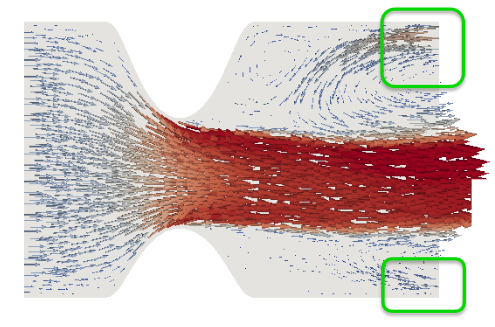
\includegraphics[width=0.6\textwidth]{Media/backflowareas.png}
  \end{figure}
\end{frame}
\begin{frame}{What is backflow and why does it occur?}
    Often occurs in physiological systems (cardiovascular, respiratory, etc)
    \begin{figure}[h]
     \centering
     \begin{subfigure}[b]{0.3\textwidth}
         \centering
         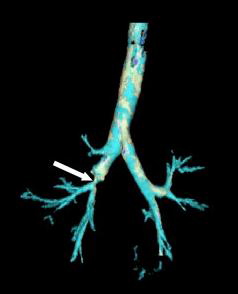
\includegraphics[width=\textwidth]{Media/Stenosis1.png}
        %  \caption{small gamma}
        %  \label{fig:smallg2}
     \end{subfigure}
     \hfill
     \begin{subfigure}[b]{0.3\textwidth}
         \centering
         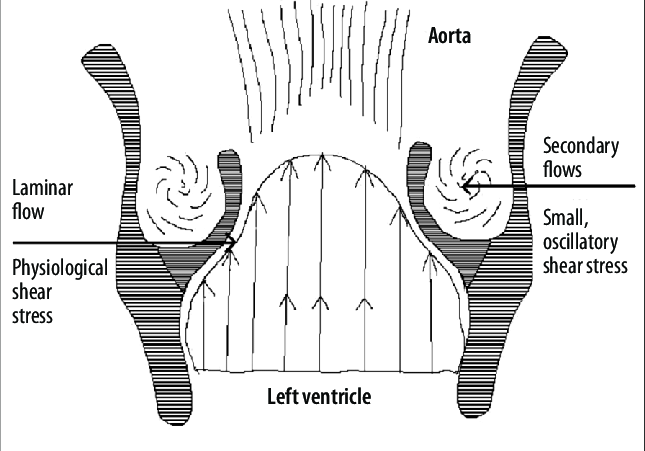
\includegraphics[width=\textwidth]{Media/Stenosis2.png}
        %  \caption{large gamma}
        %  \label{fig:highg2}
     \end{subfigure}
      \hfill
     \begin{subfigure}[b]{0.3\textwidth}
         \centering
         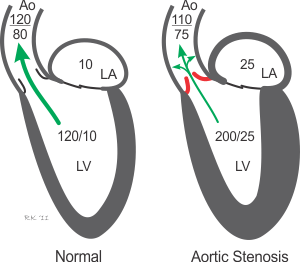
\includegraphics[width=\textwidth]{Media/Stenosis3.png}
        %  \caption{large gamma}
        %  \label{fig:highg2}
     \end{subfigure}
        % \caption{different stabilisation with different gamma's}
        % \label{fig:2 three graphs}
\end{figure}

\end{frame}
% \begin{frame}{Where does backflow occur?}
%   Some temp text
% \end{frame}
\begin{frame}{Why do we need to stabilise backflow?}
%   Would want to numerically model these physiological systems as less invasive then surgery, however 
  Regions of backflow along a boundary can cause numerical instability, resulting in incorrect solutions, wasting computational time, etc
  \begin{figure}[b]
      \centering
      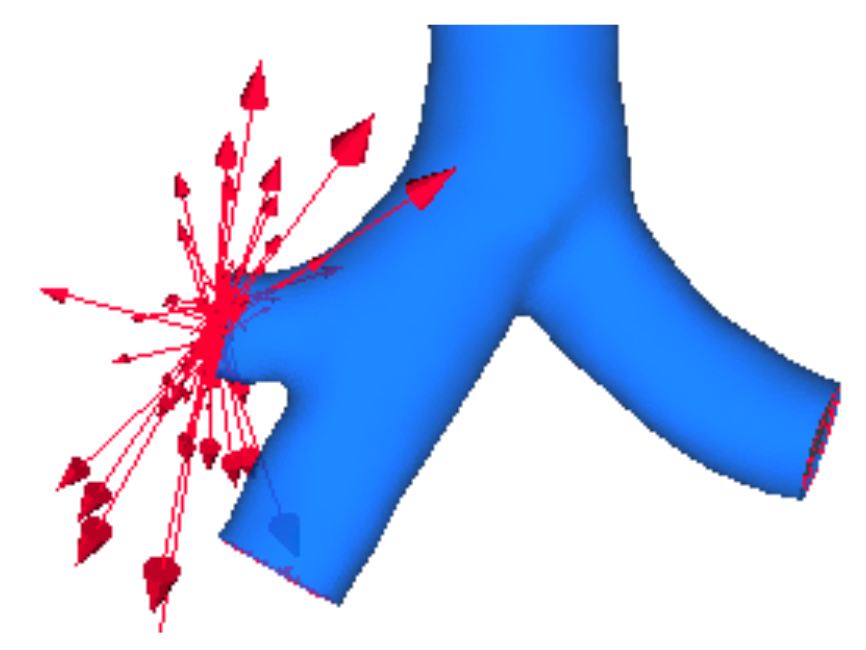
\includegraphics[width=0.4\textwidth]{Media/instability.PNG}
  \end{figure}
\end{frame}
\begin{frame}{Backflow instability example}
      \begin{center}
\includemedia[
    activate=onclick,
    % activate=pageopen,
    passcontext,
    transparent,
    width=0.75\textwidth,
]{
\includegraphics{Movies/cover.png}}{Movies/nostab.swf}
\end{center}
\end{frame}
% \begin{frame}{Mathematical foundation for backflow}

% \end{frame}
\begin{frame}{Backflow in Navier-Stokes}

\begin{block}{Navier-Stokes Equations}
\[\begin{aligned}
 \rho\partial_t\bmu + \rho(\bmu - \textbf{w})\cdot\nabla\bmu - 2\mu\nabla\cdot\epsilon(\bmu) + \nabla p &= 0 \\ \nabla\cdot\bmu &= 0 
\end{aligned}\]
\end{block}

Changing to weak form, and testing with the solution, \(\bmu\), the NS equations can be rewritten as:
\[\footnotesize
\partial_t\frac{\rho}{2}\fint\norm{\bmu}^2 = -2\mu \fint \norm{\varepsilon(\bmu)}^2 - \underbrace{\frac{\rho}{2}\bint\bmu\cdot\bmn\norm{\bmu}^2}_{\text{\huge \textasteriskcentered}}
\]


\end{frame}
\begin{frame}{Stabilising Backflow}
  
  \begin{block}{Stabilisation types}
  \begin{itemize}
      \item Velocity Penalisation:
      \(
      S = \beta\frac{\rho}{2}\bint \abs{\bmu \cdot \bmn }_- \bmu \cdot \bmv
      \)
      \item Tangential Derivative Penalisation:
      \begin{itemize}
          \item  \(      S = \gamma U_b h^2 \frac{\rho}{2} \bint \qty(t^{T}\nabla\bmu \cdot t^{T}\nabla\bmv), \qquad U_b = \max \abs{\bmu \cdot \bmn}_-\)
      \item \(
      S = \gamma\frac{\rho}{2}h^{2}\bint \abs{\bmu \cdot \bmn }_- \qty(t^{T}\nabla\bmu \cdot t^{T}\nabla\bmv)
      \)
      \end{itemize}
     
  \end{itemize}
      
  \end{block}
\end{frame}
\subsection{Problem Description}
\begin{frame}{Main Question}
\begin{center}
    \textbf{"Can these parameters be automatically chosen either at the beginning of- or during the computation such that stability is maintained while possibly improving the accuracy of the solution"}
\end{center}
\end{frame}